\documentclass[a4paper,12pt]{article}
\usepackage[utf8]{inputenc}
\usepackage[english,russian]{babel}

\usepackage{setspace}
\onehalfspacing

\usepackage{graphicx}
%\graphicspath{{pictures/}}
\DeclareGraphicsExtensions{.pdf,.png,.jpg}

\usepackage{longtable}
\usepackage{pdflscape}
\usepackage{mathptmx}

%\usepackage{natbib}

\usepackage{geometry}
\geometry{top=20mm}
\geometry{bottom=20mm}
\geometry{left=25mm}
\geometry{right=20mm}

%%\usepackage{biblatex}
%%\addbibresource{ref.bib}
%\bibliographystyle{plain}
%\bibliography{ref.bib}
\usepackage{apacite}

\begin{document}
	
\begin{center}
	Федеральное государственное автономное образовательное учреждение высшего образования «Национальный исследовательский университет «Высшая школа экономики»
	\\
	\bigskip
	Санкт-Петербургская Школа экономики и менеджмента \\
	Образовательная Программа "Экономика"
\end{center}

\vspace{8em}

\begin{center}
	{\Large КУРСОВАЯ РАБОТА}\\
	\textsc{\textbf{
			На тему
			\linebreak
			"Применение гравитационной модели к анализу миграций в Российской империи"}}
\end{center}

\vspace{2em}

\hfill\parbox{16cm}{
	\hspace*{5cm}\hspace*{-5cm}Выполнил студент группы БЭК-182\\
	Соснин Юрий Алексеевич\\
	
	\hspace*{5cm}\hspace*{-5cm}Научный руководитель:\\
	ст.преп. Куга Яков Тойвович\\
}

\vspace{\fill}

\begin{center}
	Санкт-Петербург
	
	2021 г.
\end{center}
\thispagestyle{empty}

\clearpage

\tableofcontents

\clearpage
\section{Введение}

что-то


\clearpage
\section{Гравитационная модель}

\subsection{История гравитации}

Впервые основные гипотезы пространственного моделирования миграций предложил в 1885 году британский географ и статистик Эрнст Георг Равенштайн в знаменитой статье The Laws of Migration в Journal of the Royal Statistical Society. (…) Автор анализирует данные британских переписей 1871 и 1881 годов, определяя основные направления и силу потоков внутренней миграции между Англией, Шотландией и Ирландией, а также между графствами внутри этих королевств. Равенштайн не предложил математической модели миграции, его анализ напоминает скорее современную описательную статистику, однако на основе своих наблюдений он сформулировал несколько гипотез, «законы миграции». 

Во-первых, Равенштайн отмечает, что основная причина миграции – рынок труда. Жители Британии чаще переселялись в торговые и промышленные центры, с большими возможностями трудоустройства и …

Во-вторых, автор отмечает отрицательную роль расстояния и других пространственных характеристик в силе миграционных потоков. В первую очередь, города привлекают жителей близлежащей сельской местности, потом – жителей соседних графств, и, наконец, жителей остальной страны (морское сообщение, при этом, также способствует миграции.) Сама сила миграционного потока также, очевидно, зависит от населения, готового принимать в нем участие.

С другой стороны, даже между самыми дальними регионами есть двустороннее миграционное «сообщение». Каждый поток имеет противоположный.

Наконец, мигранты имеют особые характеристики: молодые, не имеющие детей, и жители деревень более предрасположены к миграции, чем, соответственно, более взрослые, жители города и семьи с детьми. Кроме того, в случае Британии 19 века, женщины более мобильны, чем мужчины. Эти рассуждения задают основу последующим моделям, определяя миграцию как селективный процесс.

Работа Равенштайна оказала значительное влияние на будущие работы демографов, социологов, и, в конечном счете, экономистов, определив основные гипотезы для моделей миграции и пространственного взаимодействия в целом. 

Американский социолог Самуэль Стоффер в статье «Intervening opportunities: a theory relating mobility and distance» продолжил развивать идею о влиянии расстояния на миграционные потоки. Согласно его тории, не cтолько расстояние имеет значение, сколько так называемые вмешивающиеся обстоятельства (intervening opportunities) – транспортные расходы, информация о месте назначения, законодательное барьеры, культурные отличия и так далее.

Гравитационная модель – модель пространственного социального взаимодействия - впервые была сформулирована John Q. Stewart в 1948 году, как аналогия физическому закону Ньютона. (John Q. Stewart, 1948) Вся статья пронизана физическими аналогиями: например, отдельные люди сравниваются с молекулами газа, а большие группы людей – с самим газом. На этом основании он критикует получивших распространение к тому времени микро-подход, изучающий отдельных людей и их мотивацию – если бы физики изучали только молекулы, законов, описывающих свойство газов, не существовало бы.


\subsection{Методы оценки}

ppml

\subsection{Гравитацонные модели в истории}

эээ

ikfyuik

\subsection{Гравитацонные модели в развивающихся странах}

kjhgf

jkhg

\clearpage
\section{Российская империя в 19 веке}

ri

\clearpage
\section{Данные, модель и гипотезы}

\subsection{Данные}

впрыкеиыеи

\subsection{Гипотезы}

123

\subsection{Результаты}

results

\clearpage
\section{Заключение}

ending. \cite{anderson_internal_1980}
asd. \cite{leasure_internal_1968}

%\bibliographystyle{plain}
%\bibliography{ref.bib}
%\printbibliography

\clearpage

\bibliographystyle{apacite}
\bibliography{ref}
	
\clearpage\appendix
\section{Таблицы}

{
\def\sym#1{\ifmmode^{#1}\else\(^{#1}\)\fi}
\begin{longtable}{l*{4}{c}}
\hline\hline\endfirsthead\hline\endhead\hline\endfoot\endlastfoot
            &\multicolumn{1}{c}{(1)}&\multicolumn{1}{c}{(2)}&\multicolumn{1}{c}{(3)}&\multicolumn{1}{c}{(4)}\\
            &\multicolumn{1}{c}{Simple}&\multicolumn{1}{c}{Industry shares}&\multicolumn{1}{c}{Industry outputs}&\multicolumn{1}{c}{No density}\\
\hline
log\_pop\_i   &       0.927\sym{***}&       0.860\sym{***}&       0.794\sym{***}&       0.973\sym{***}\\
log\_pop\_j   &       0.523\sym{***}&       1.176\sym{***}&       1.113\sym{***}&       0.472\sym{***}\\
log\_dist    &      -1.204\sym{***}&      -1.067\sym{***}&      -1.024\sym{***}&      -0.801\sym{***}\\
borders     &                     &       0.994\sym{***}&       1.030\sym{***}&       1.220\sym{***}\\
sea\_i       &                     &      0.0425         &      0.0465         &      -0.418\sym{***}\\
sea\_j       &                     &      0.0638         &      -0.226\sym{*}  &       0.726\sym{***}\\
log\_lit\_i   &                     &       0.162\sym{*}  &       0.188\sym{*}  &       0.320\sym{***}\\
log\_lit\_j   &                     &     -0.0602         &       0.242\sym{**} &      -0.303\sym{***}\\
log\_urb\_i   &                     &      0.0825         &      -0.222\sym{*}  &       0.207         \\
log\_urb\_j   &                     &       0.572\sym{***}&       1.367\sym{***}&       0.145         \\
log\_r\_i     &                     &      -0.297\sym{**} &      -0.349\sym{***}&     -0.0942         \\
log\_r\_j     &                     &       0.984\sym{***}&       1.057\sym{***}&       0.785\sym{***}\\
log\_den\_i   &                     &       0.509\sym{***}&       0.559\sym{***}&                     \\
log\_den\_j   &                     &      -0.986\sym{***}&      -0.980\sym{***}&                     \\
log\_ind\_share\_i&                     &      0.0124         &                     &       0.181         \\
log\_ind\_share\_j&                     &     -0.0309         &                     &      -0.176         \\
log\_agr\_share\_i&                     &       0.683\sym{*}  &                     &       1.010\sym{**} \\
log\_agr\_share\_j&                     &      -1.568\sym{***}&                     &      -1.749\sym{***}\\
log\_serfs\_i &                     &     -0.0263         &     -0.0101         &     -0.0413         \\
log\_serfs\_j &                     &      -0.123\sym{***}&      -0.132\sym{***}&      -0.170\sym{***}\\
log\_russian\_abs&                     &     -0.0503\sym{**} &     -0.0596\sym{**} &     -0.0575\sym{**} \\
log\_polish\_abs&                     &     -0.0339         &     -0.0310         &     -0.0536\sym{*}  \\
log\_jewish\_abs&                     &     -0.0243         &     -0.0388         &     -0.0492         \\
log\_german\_abs&                     &      0.0329         &      0.0263         &      0.0361         \\
capital\_i   &                     &      -0.206         &      -0.556\sym{**} &       0.380         \\
capital\_j   &                     &       0.622\sym{**} &       1.599\sym{***}&       0.285         \\
tmp\_diff    &                     &      0.0690\sym{***}&      0.0590\sym{***}&     -0.0962\sym{***}\\
wet\_diff    &                     &      -0.136\sym{***}&      -0.113\sym{***}&      -0.166\sym{***}\\
pre\_diff    &                     &      0.0349\sym{***}&      0.0381\sym{***}&      0.0149\sym{***}\\
log\_ind\_i   &                     &                     &     -0.0175         &                     \\
log\_ind\_j   &                     &                     &     -0.0742         &                     \\
log\_agr\_i   &                     &                     &      0.0256         &                     \\
log\_agr\_j   &                     &                     &      -0.141\sym{***}&                     \\
\_cons      &      -5.141\sym{***}&      -12.79\sym{***}&      -9.254\sym{***}&      -8.398\sym{***}\\
\hline
\(N\)       &        7832         &        7482         &        6972         &        7482         \\
\hline\hline
\multicolumn{5}{l}{\footnotesize \sym{*} \(p<0.05\), \sym{**} \(p<0.01\), \sym{***} \(p<0.001\)}\\
\end{longtable}
}

\clearpage

\begin{landscape}

\section{Карты}

\begin{figure}[h!]
	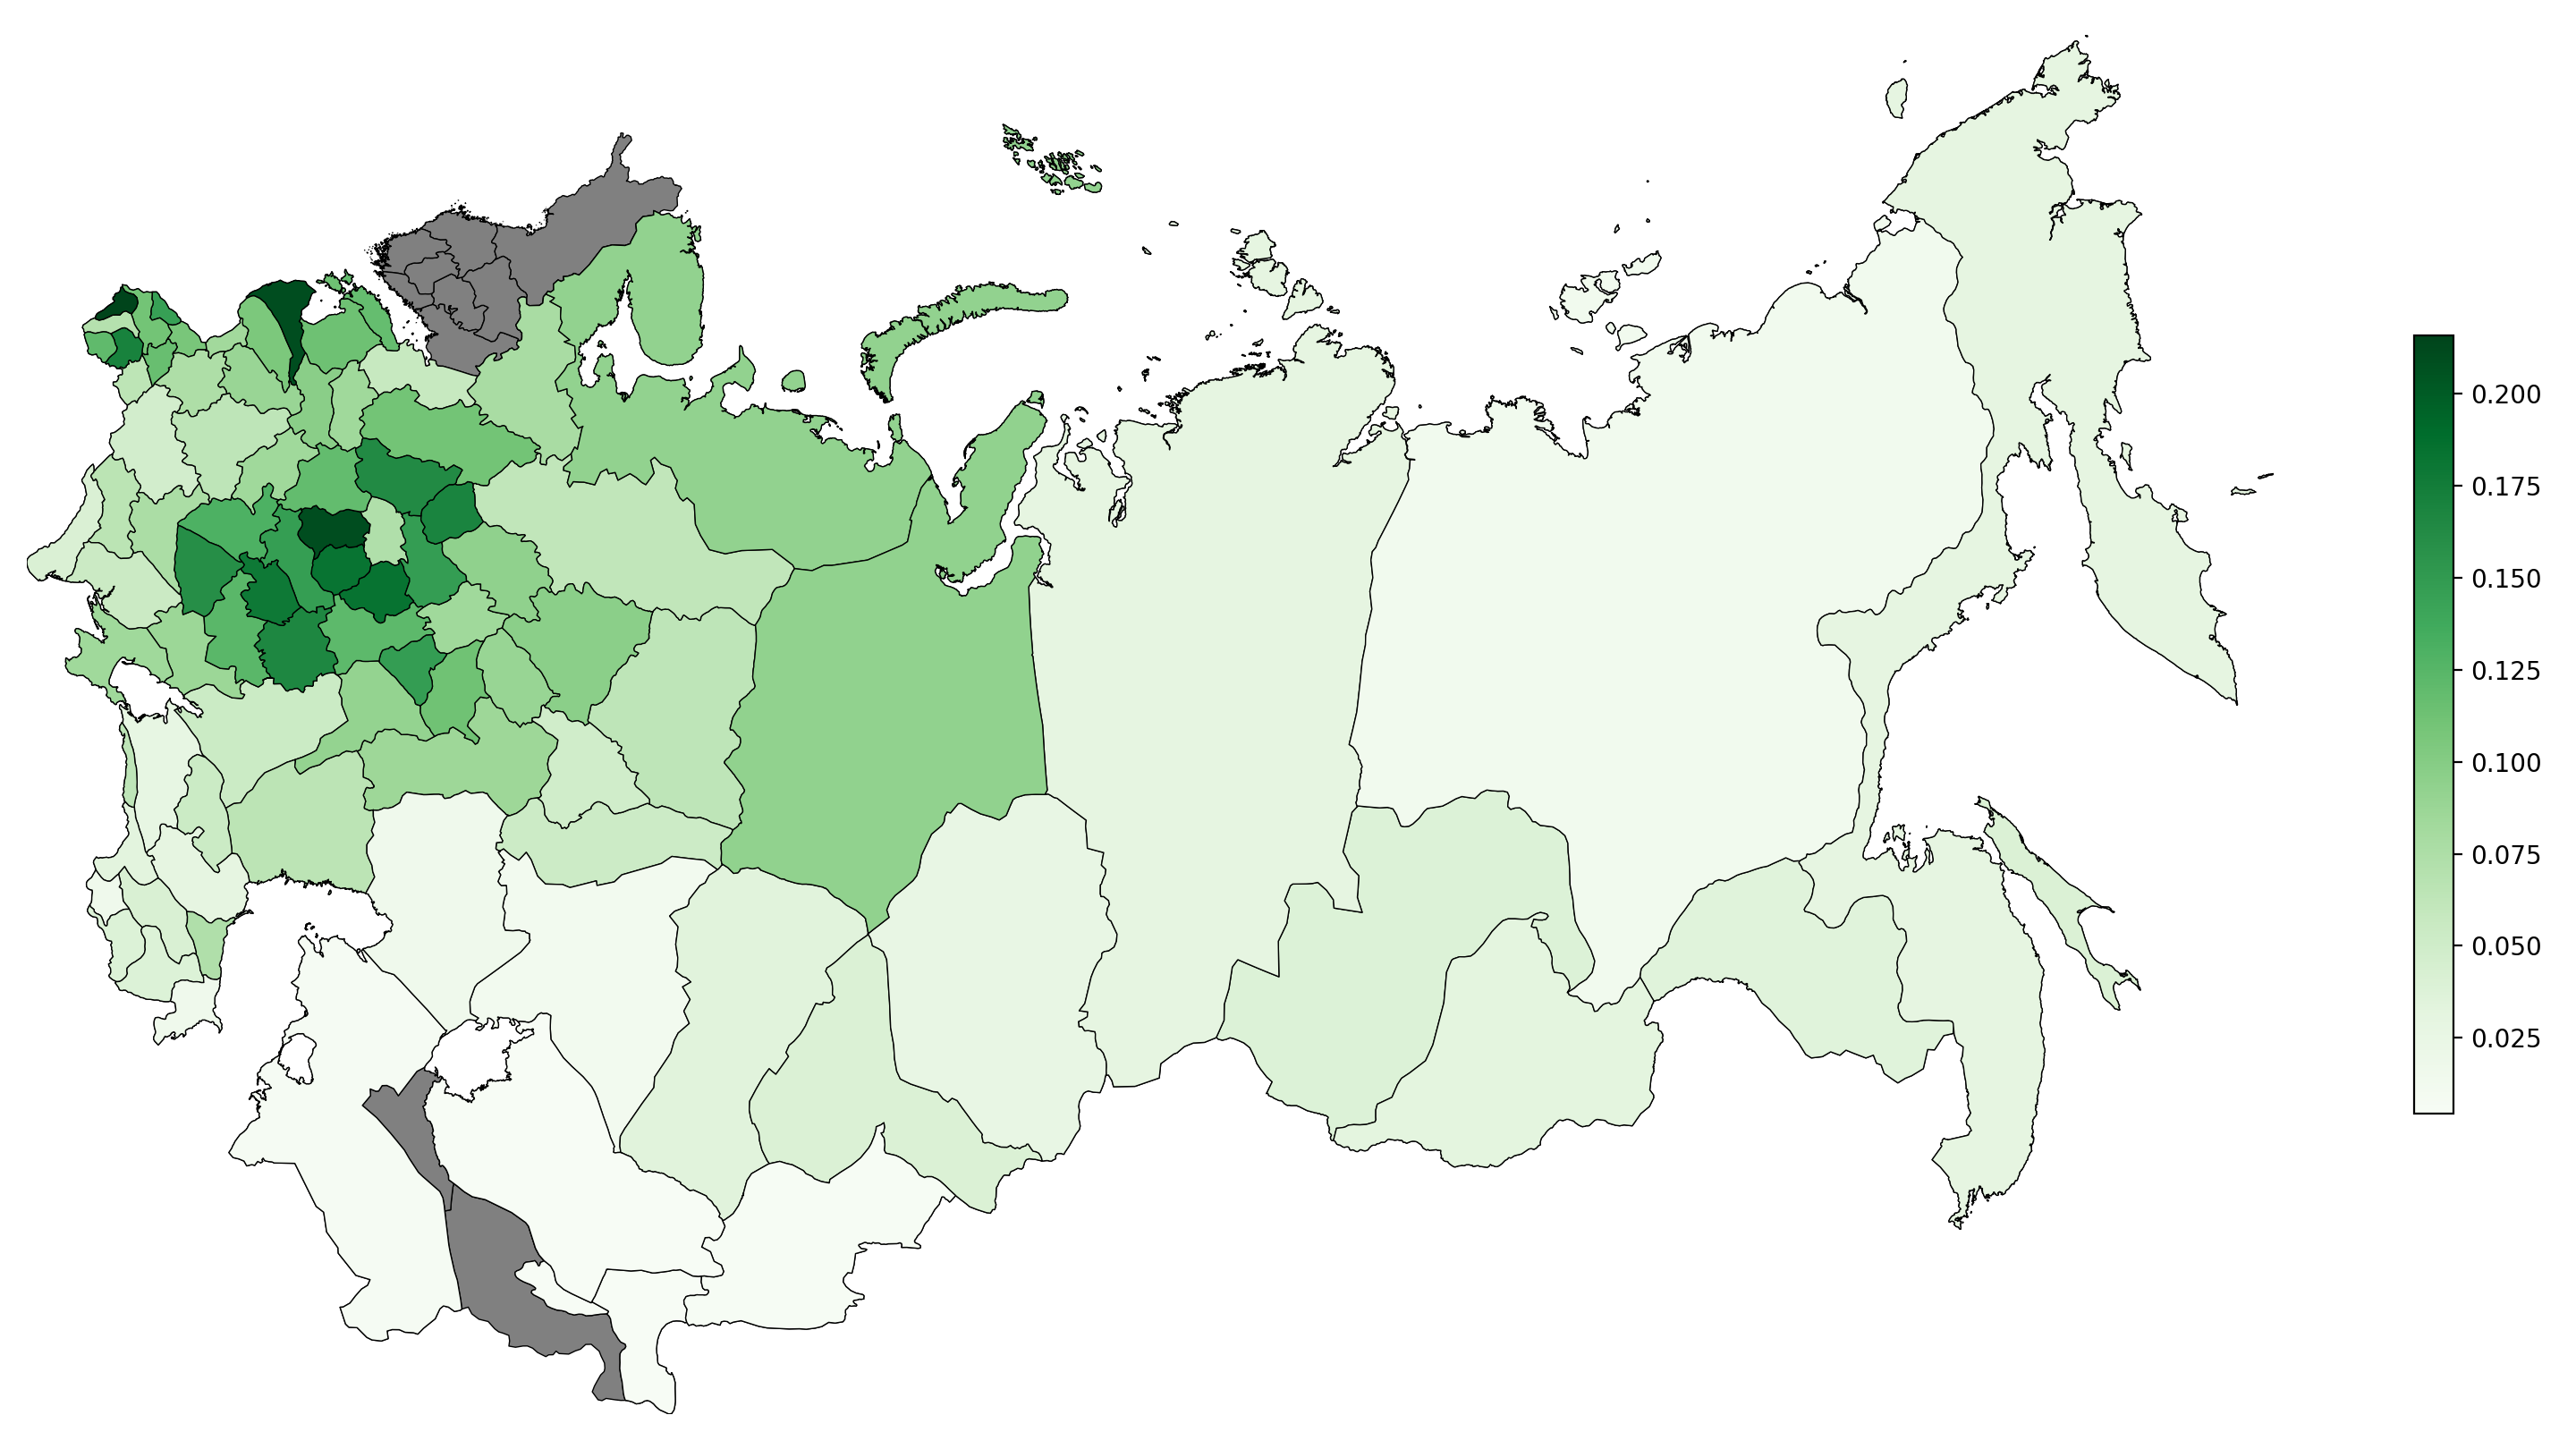
\includegraphics[height=0.85\textwidth]{pics/mig_of_pop_from.png}
	\caption{Родившихся в регионе, но проживающих в других регионах, доля населения}
	\label{fig:image1}
\end{figure}
	
\begin{figure}[h!]
	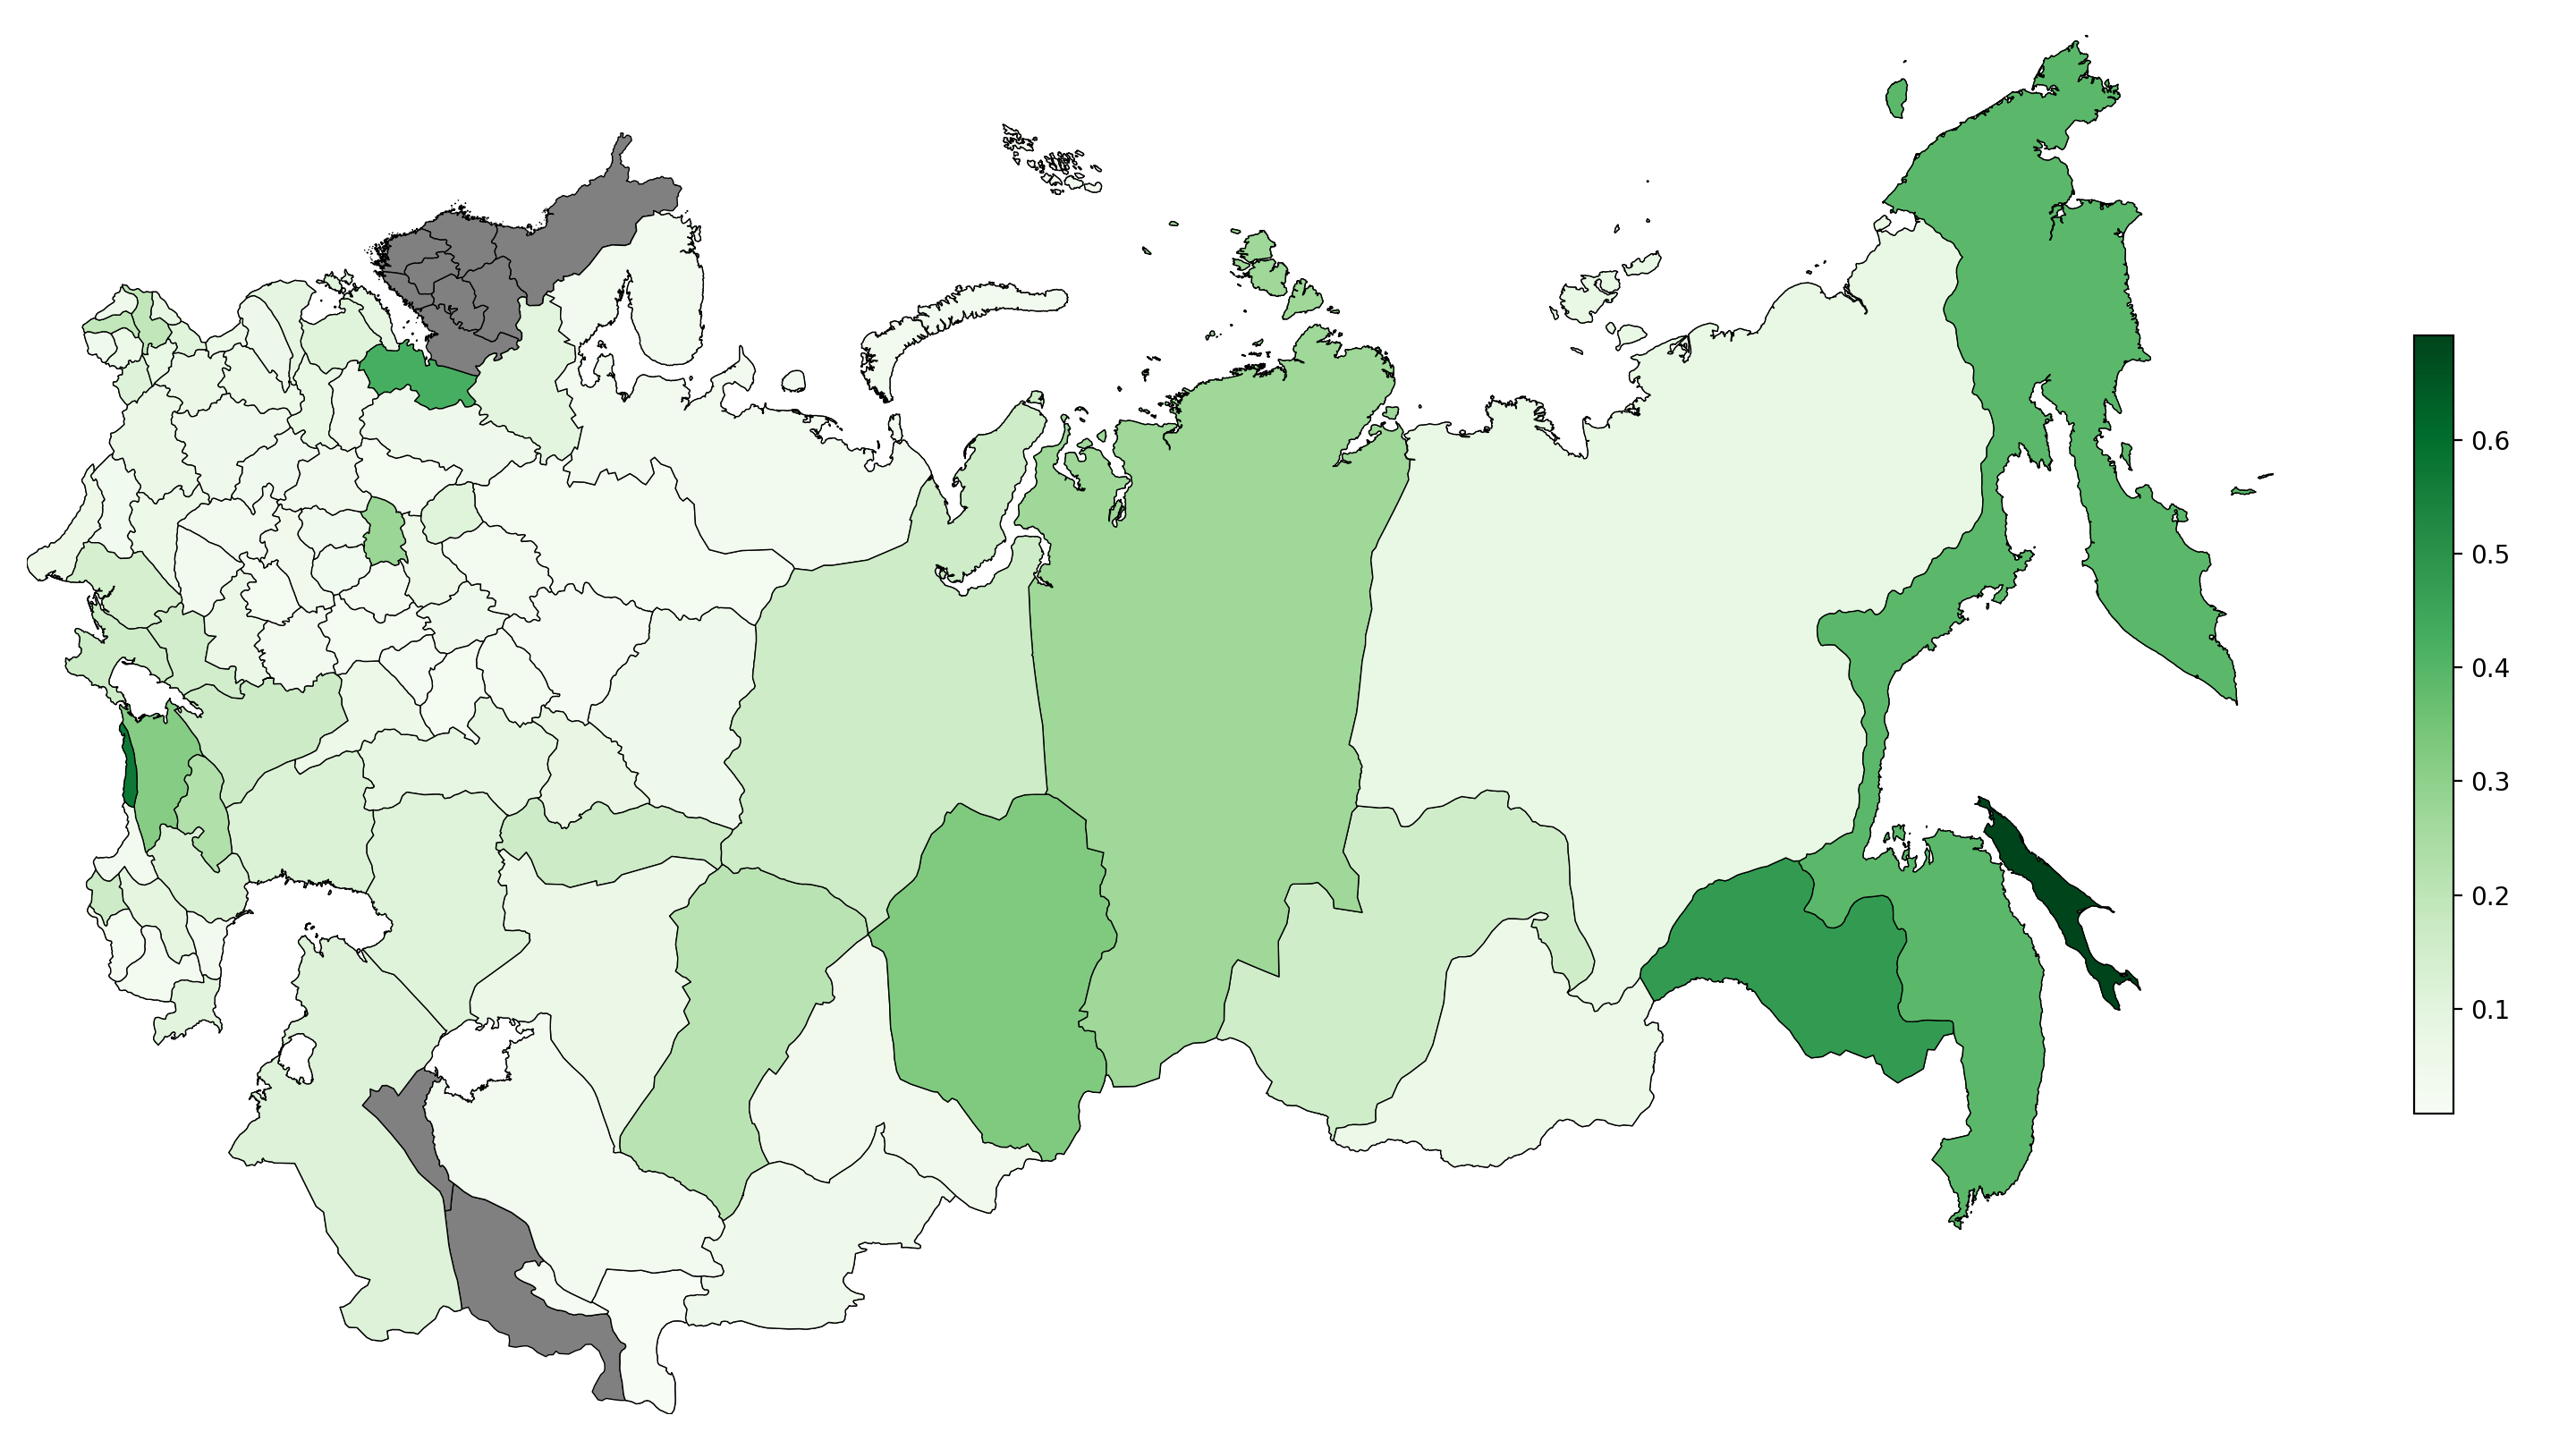
\includegraphics[height=0.85\textwidth]{pics/mig_of_pop_to.png}
	\caption{Родившихся в других регионах, но проживающих в этом, доля населения}
	\label{fig:image1}
\end{figure}

\end{landscape}


\end{document}

